\documentclass[12pt]{article}
\usepackage{amsmath}
\usepackage{graphicx}
\usepackage{geometry}
\usepackage{listings}
\usepackage{xcolor}

\geometry{margin=1in}

\title{Design and Implementation of Universal Shift Register using Verilog}
\author{}
\date{}

\lstset{
    language=Verilog,
    basicstyle=\ttfamily\small,
    keywordstyle=\color{blue},
    commentstyle=\color{green},
    stringstyle=\color{red},
    breaklines=true,
    frame=single
}

\begin{document}

\maketitle

\section{Introduction}

A Universal Shift Register is a sequential digital circuit capable of performing multiple operations such as:
\begin{itemize}
    \item Shift Left
    \item Shift Right
    \item Parallel Load
    \item Hold (No Operation)
\end{itemize}

Unlike simple shift registers, a universal shift register provides flexibility by supporting both serial and parallel data transfer. It is widely used in digital systems such as microprocessors, data storage systems, communication interfaces, and arithmetic logic units.

The implementation of such a register using Verilog Hardware Description Language (HDL) allows simulation, synthesis, and efficient hardware realization using FPGA or ASIC technologies.

\section{Components Needed}

The following components are required for designing a Universal Shift Register:

\begin{itemize}
    \item Flip-Flops (D Flip-Flops are commonly used)
    \item Multiplexers (for selecting operations)
    \item Clock signal
    \item Control inputs (mode selection)
    \item Serial input lines (left and right)
    \item Parallel input lines
\end{itemize}

In Verilog implementation, these components are modeled using behavioral or structural constructs rather than physical components.

\section{Inputs and Outputs}

\subsection{Inputs}
\begin{itemize}
    \item clk : Clock signal
    \item reset : Reset signal (synchronous or asynchronous)
    \item mode[1:0] : Control signal to select operation
    \item data\_in[3:0] : Parallel input data
    \item serial\_in\_left : Serial input for left shift
    \item serial\_in\_right : Serial input for right shift
\end{itemize}

\subsection{Outputs}
\begin{itemize}
    \item data\_out[3:0] : Output of the register
\end{itemize}

\section{Truth Table}

\begin{center}
\begin{tabular}{|c|c|l|}
\hline
Mode & Operation & Description \\
\hline
00 & Hold & No change in output \\
01 & Shift Right & Bits shift right, MSB gets serial\_in\_left \\
10 & Shift Left & Bits shift left, LSB gets serial\_in\_right \\
11 & Parallel Load & Load data\_in into register \\
\hline
\end{tabular}
\end{center}

\subsection{State Representation}

Let the current state be $Q = [Q_3 Q_2 Q_1 Q_0]$

\begin{itemize}
    \item Shift Right: $Q \leftarrow [serial\_in\_left, Q_3, Q_2, Q_1]$
    \item Shift Left: $Q \leftarrow [Q_2, Q_1, Q_0, serial\_in\_right]$
    \item Parallel Load: $Q \leftarrow data\_in$
    \item Hold: $Q \leftarrow Q$
\end{itemize}

\subsection{Circuit Diagram}

\begin{center}
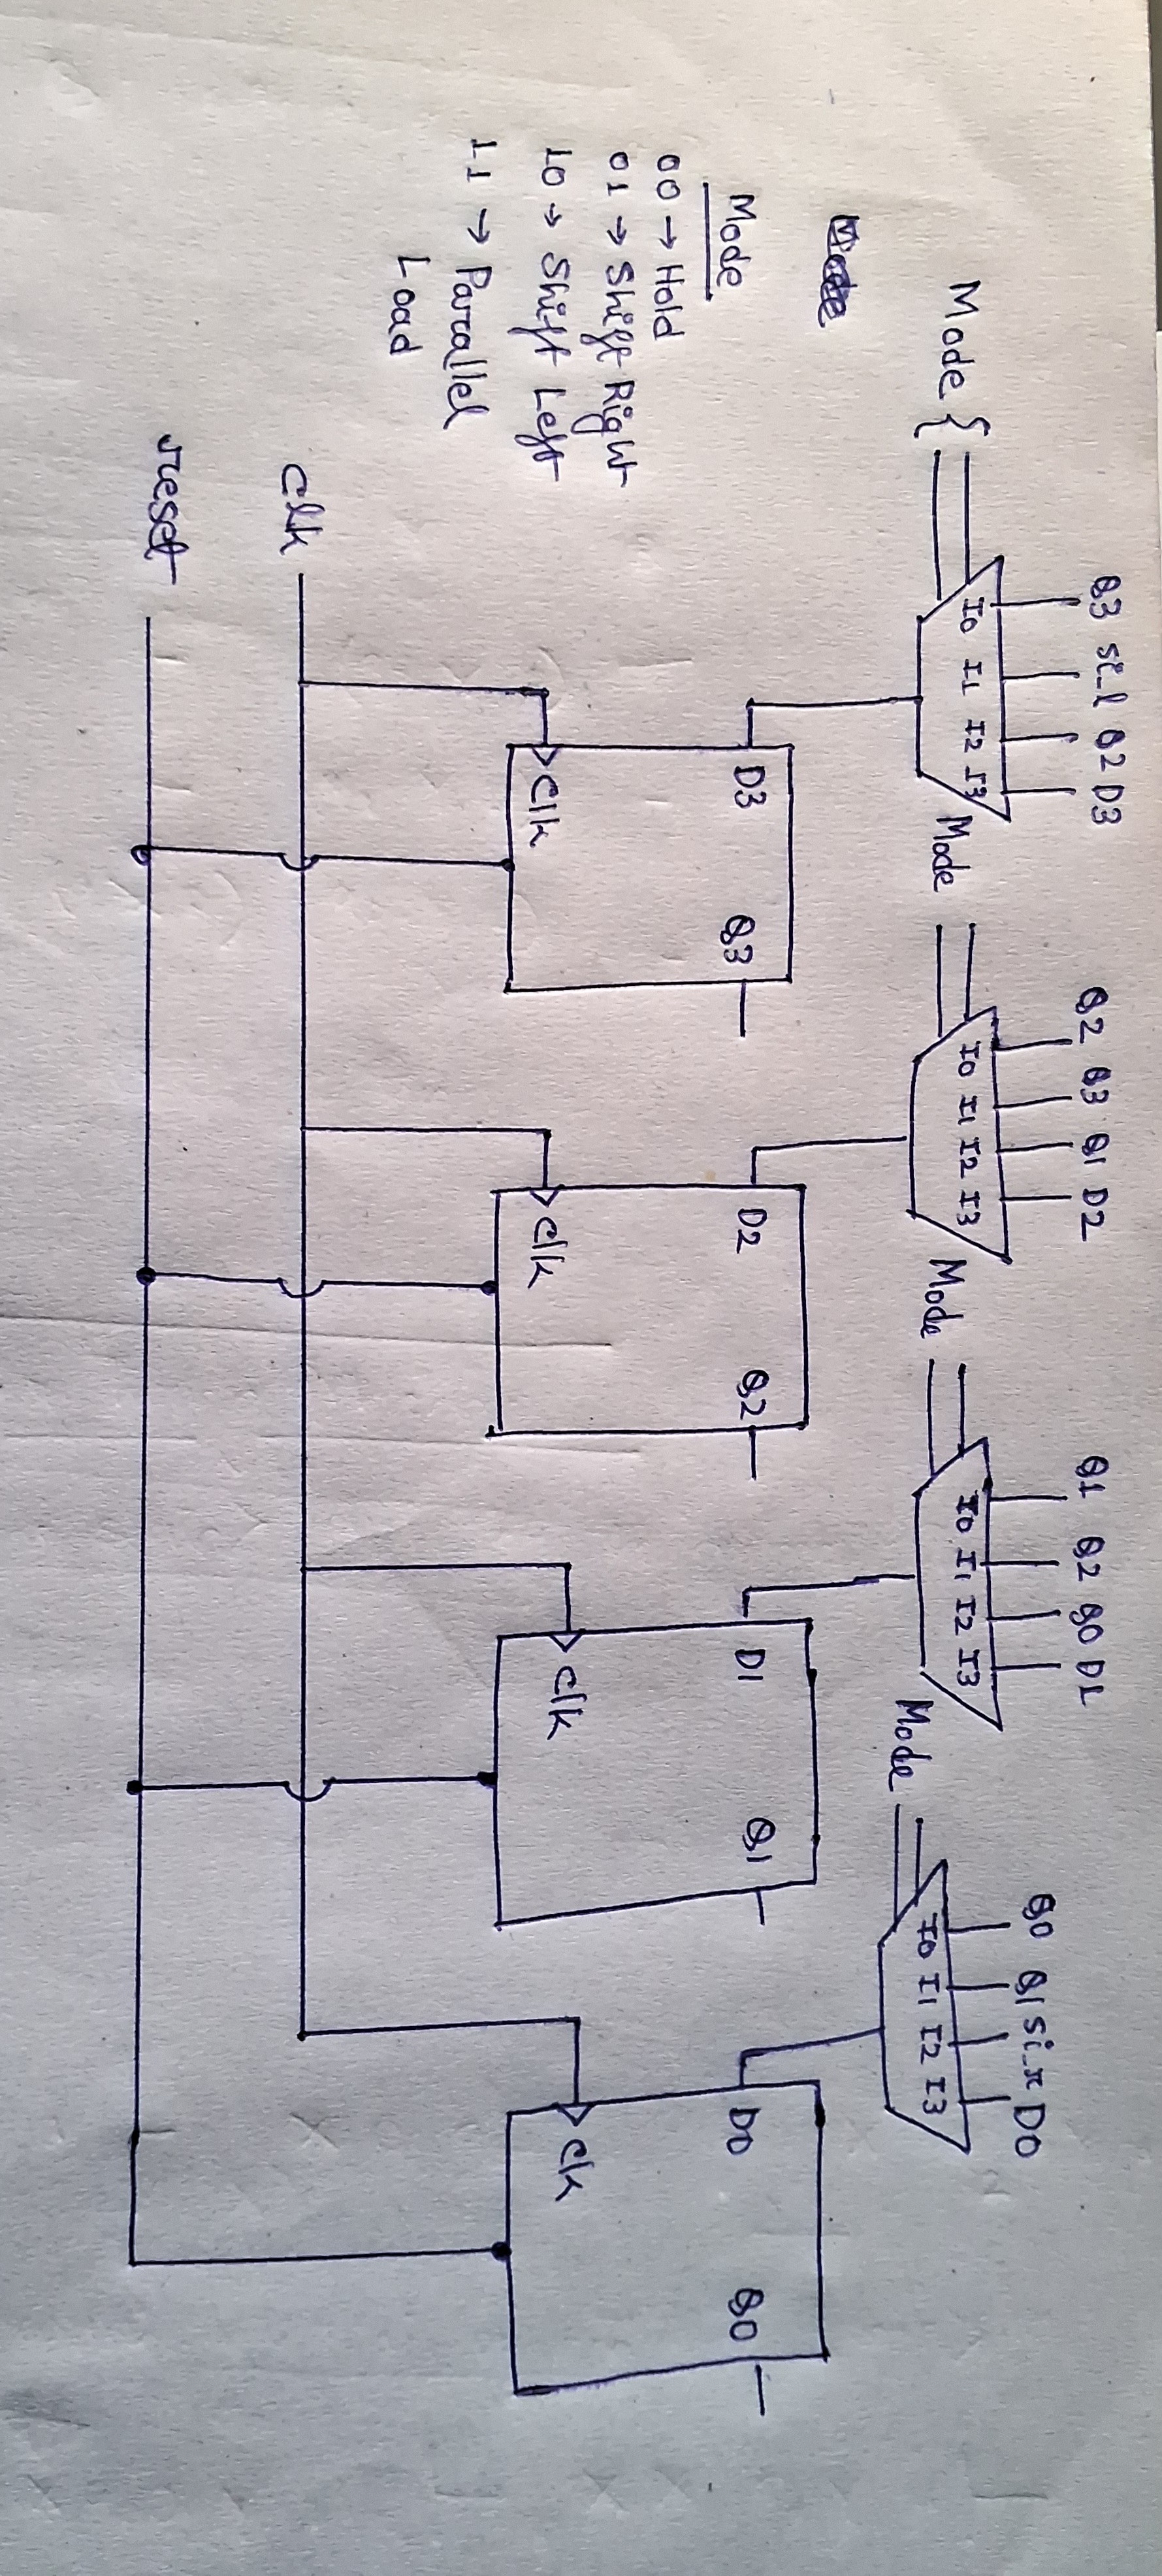
\includegraphics[width=0.4\textwidth, angle=90]{ckt_diagram.jpg}
\end{center}

\section{Working Principle}

The Universal Shift Register operates based on the control signal \texttt{mode[1:0]} which determines the functionality at each clock pulse.

\begin{itemize}
    \item \textbf{Hold (00):} The register maintains its previous state. No data movement occurs.
    
    \item \textbf{Shift Right (01):} Each bit shifts one position to the right. The leftmost bit (MSB) is filled by the serial input \texttt{serial\_in\_left}.
    
    \item \textbf{Shift Left (10):} Each bit shifts one position to the left. The rightmost bit (LSB) is filled by the serial input \texttt{serial\_in\_right}.
    
    \item \textbf{Parallel Load (11):} All bits of the register are simultaneously updated with the parallel input \texttt{data\_in}.
\end{itemize}

The operation is synchronized with the clock signal. On each rising edge of the clock, the selected operation is executed.

Reset initializes the register to a known state (usually zero).

\section{Verilog Design Code}

\begin{lstlisting}
module universal_shift_register(
    input clk,
    input reset,
    input [1:0] mode,
    input [3:0] data_in,
    input serial_in_left,
    input serial_in_right,
    output reg [3:0] data_out
);

always @(posedge clk or posedge reset) begin
    if (reset)
        data_out <= 4'b0000;
    else begin
        case(mode)
            2'b00: data_out <= data_out; // Hold
            2'b01: data_out <= {serial_in_left, data_out[3:1]}; // Shift Right
            2'b10: data_out <= {data_out[2:0], serial_in_right}; // Shift Left
            2'b11: data_out <= data_in; // Parallel Load
        endcase
    end
end

endmodule
\end{lstlisting}

\section{Testbench Code}

\begin{lstlisting}
module tb_universal_shift_register;

reg clk;
reg reset;
reg [1:0] mode;
reg [3:0] data_in;
reg serial_in_left;
reg serial_in_right;
wire [3:0] data_out;

universal_shift_register uut (
    .clk(clk),
    .reset(reset),
    .mode(mode),
    .data_in(data_in),
    .serial_in_left(serial_in_left),
    .serial_in_right(serial_in_right),
    .data_out(data_out)
);

always #5 clk = ~clk;

initial begin
    clk = 0;
    reset = 1;
    #10 reset = 0;

    mode = 2'b11;
    data_in = 4'b1010;
    #10;

    mode = 2'b01;
    serial_in_left = 1;
    #10;

    mode = 2'b10;
    serial_in_right = 0;
    #10;

    mode = 2'b00;
    #10;

    $finish;
end

endmodule
\end{lstlisting}

\section{Code Explanation}

\subsection{Design Code Explanation}

\begin{itemize}
    \item The module implements a 4-bit universal shift register using behavioral modeling in Verilog.
    
    \item The \texttt{always} block is sensitive to the rising edge of the clock and the reset signal:
    \begin{itemize}
        \item On \texttt{reset = 1}, the register is initialized to \texttt{0000}.
        \item On each rising edge of \texttt{clk}, the operation is selected based on the \texttt{mode} input.
    \end{itemize}
    
    \item The \texttt{mode[1:0]} input determines the operation:
    \begin{itemize}
        \item \texttt{00} : Hold (no change in output)
        \item \texttt{01} : Shift Right
        \item \texttt{10} : Shift Left
        \item \texttt{11} : Parallel Load
    \end{itemize}
    
    \item The concatenation operator \texttt{\{\}} is used to implement shifting:
    \begin{itemize}
        \item Shift Right: \texttt{\{serial\_in\_left, data\_out[3:1]\}}
        \item Shift Left: \texttt{\{data\_out[2:0], serial\_in\_right\}}
    \end{itemize}
    
    \item During shift operations:
    \begin{itemize}
        \item In Shift Right, the most significant bit (MSB) is filled with \texttt{serial\_in\_left}, and all bits move one position to the right.
        \item In Shift Left, the least significant bit (LSB) is filled with \texttt{serial\_in\_right}, and all bits move one position to the left.
    \end{itemize}
    
    \item All operations are synchronous, ensuring that the output changes only at the rising edge of the clock, avoiding glitches and ensuring stable sequential behavior.
\end{itemize}

\subsection{Testbench Explanation}

\begin{itemize}
    \item The testbench initializes all input signals to avoid undefined (\texttt{X}) states, ensuring accurate simulation results.
    
    \item A clock signal is generated using an \texttt{always} block that toggles every 5 time units, resulting in a clock period of 10 time units.
    
    \item Waveform dumping is enabled using:
    \begin{itemize}
        \item \texttt{\$dumpfile("dump.vcd")}
        \item \texttt{\$dumpvars(0, tb\_universal\_shift\_register)}
    \end{itemize}
    
    \item Inputs are applied synchronously using \texttt{@(negedge clk)} to ensure they are stable before the active rising edge of the clock, satisfying setup time requirements.
    
    \item The sequence of operations performed is:
    \begin{itemize}
        \item Reset the register to \texttt{0000}
        \item Parallel Load of \texttt{1010}
        \item Shift Right with serial input \texttt{1}
        \item Shift Left with serial input \texttt{0}
        \item Hold operation
    \end{itemize}
    
    \item Each operation is executed on the subsequent rising edge of the clock, and the output is observed accordingly.
    
    \item The simulation is terminated using \texttt{\$finish}.
\end{itemize}

\section{Timing Diagram}

\begin{center}
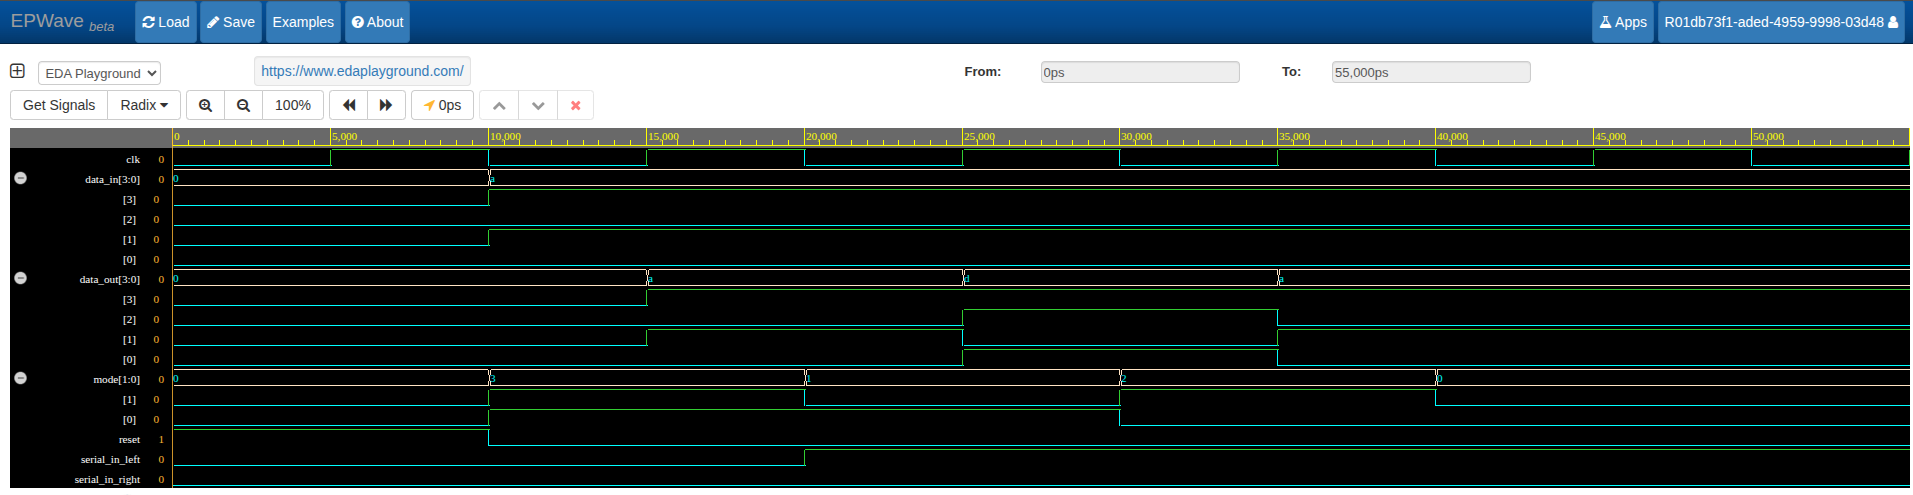
\includegraphics[width=\textwidth]{timing_diagram.png}
\end{center}

\section{Timing Diagram Explanation}

The timing diagram represents the sequential operation of the universal shift register with respect to the clock signal.

\begin{itemize}
    \item All changes in the output \texttt{data\_out} occur strictly at the rising edge of the clock, confirming correct synchronous operation.
    
    \item Initially, when \texttt{reset = 1}, the output is forced to \texttt{0000}.
    
    \item During the Parallel Load operation (\texttt{mode = 11}), the input \texttt{1010} is loaded into the register in a single clock cycle.
    
    \item During Shift Right (\texttt{mode = 01}):
    \begin{itemize}
        \item Bits move one position to the right.
        \item The MSB is filled with \texttt{serial\_in\_left}.
        \item Example: \texttt{1010 $\rightarrow$ 1101}
    \end{itemize}
    
    \item During Shift Left (\texttt{mode = 10}):
    \begin{itemize}
        \item Bits move one position to the left.
        \item The LSB is filled with \texttt{serial\_in\_right}.
        \item Example: \texttt{1101 $\rightarrow$ 1010}
    \end{itemize}
    
    \item During Hold operation (\texttt{mode = 00}), the output remains unchanged across clock cycles.
    
    \item The absence of undefined (\texttt{X}) states and the clean transitions indicate proper initialization and correct testbench design.
\end{itemize}

\section{Conclusion}

The Universal Shift Register is a versatile sequential circuit that supports multiple data operations within a single design. Using Verilog, the implementation becomes efficient, scalable, and suitable for simulation and synthesis. This design demonstrates the importance of control logic and sequential behavior in digital systems.

\end{document}